\section{A parsimonious version of the SSVI parameterization}\label{sec:svi}
The purpose of this section is to introduce a parsimonious version of the SSVI parameterization and to present some calibration results of this model on the implied volatility historical data that we considered in Section \ref{sec:empirical_study}. We start by some reminders about the SSVI parameterization of \cite{gatheral2014arbitrage}. 

% \subsection{Static arbitrages}
% An IVS is free from static arbitrage if there is no arbitrage opportunity by static trading of call and put options with prices given by inserting their implied volatility in the Black-Scholes formula. The formal definition of absence of static arbitrage is provided below.

% \begin{definition}[Absence of static arbitrage]   
% Let us denote $C_{BS}(K,T,\sigma)$ the Black-Scholes price of an European call option of strike $K$ and time-to-maturity $T$ when the constant volatility is $\sigma$. An IVS $(K,T)\mapsto \sigma_{BS}(K,T)$ is free of static arbitrage if there exists a non-negative martingale, say $(S_t)_{t\ge 0}$, on some filtered probability space $(\Omega,\mathcal{F},\mathbb{P})$ such that $C(K,T) := C_{BS}(K,T,\sigma_{BS}(K,T)) = \mathbb{E}[e^{-f_TT}(S_T-K)^+]$ for all $K,T \ge 0$ and where $f_T$ is the continuously compounded forward rate for the time-to-maturity $T$.
% \end{definition}

% \cite{roper2010arbitrage} provides sufficient conditions under which an IVS is free of static arbitrage. 
% \begin{theorem}[Theorem 2.9. from \citeauthor{roper2010arbitrage} \citeyear{roper2010arbitrage}]\label{thm:roper}
% Consider the total implied variance defined by $w(k,T) = \sigma_{BS}^2(k,T)T$ where $\sigma_{BS}(k,T)$ is the Black-Scholes implied volatility associated to the log-strike\footnote{We recall that the log-strike $k$ of a vanilla option of strike $K$ and forward price $F=S_0e^{rT}$ is defined as $k = \log \left(\frac{K}{F} \right)$} $k$ and the time-to-maturity $T$. If $w:\mathbb{R}\times \mathbb{R}_+ \rightarrow \mathbb{R}_+$ satisfies the following conditions:
% \begin{enumerate}[(i)]
%     \item $w(\cdot,T)$ is of class $C^2$ for all $T\ge 0$,
%     \item $w(k,T) >0$ for all $(k,T)\in \mathbb{R}\times\mathbb{R}_+^*$,
%     \item for each $(k,T)\in \mathbb{R}\times\mathbb{R}_+^*$, 
%     \begin{equation}
%         \left(1-\frac{k\partial_k w(k,T)}{2w(k,T)}\right)^2-\frac{\partial_k w(k,T)^2}{4}\left(\frac{1}{w(k,T)}+\frac{1}{4} \right)+\frac{\partial^2_{kk}w(k,T)}{2} \ge 0,
%     \end{equation}
%     \item $w(k,\cdot)$ is non-decreasing for each $k\in \mathbb{R}$,
%     \item $-k/\sqrt{w(k,T)}+\sqrt{w(k,T)}/2\underset{k\to +\infty}{\rightarrow}-\infty$ for all $T>0$ and,
%     \item $w(k,0)=0$ for all $k\in \mathbb{R}$, 
% \end{enumerate}
% then the total implied variance surface $w$ is free of static arbitrage. 
% \end{theorem}

% \begin{remark}
% An IVS is said to be free of butterfly arbitrage if conditions $(iii)$ and $(v)$ are satisfied and it is said to be free of calendar spread arbitrage if condition $(iv)$ is satisfied. To our knowledge, this terminology is due to \cite{gatheral2014arbitrage}.
% \end{remark}

\subsection{The SSVI parameterization}\label{sec:ssvi}
Devised at Merill Lynch in 1999 and publicly disseminated by \cite{gatheral2004parsimonious}, the Stochastic Volatility Inspired (SVI) parameterization is a popular parameterization of the implied volatility smile. To be more precise, it is a parameterization of the total implied variance, defined by $w(k,T):=\sigma_{BS}^2(k,T)T$ where $\sigma_{BS}(k,T)$ is the Black-Scholes implied volatility associated to the log-strike\footnote{We recall that the log-strike $k$ of a vanilla option of strike $K$ and forward price $F=S_0e^{f_T T}$ is defined as $k = \log \left(\frac{K}{F} \right)$} $k$ and the time-to-maturity $T$. The popularity of this parameterization is mainly due to its tractability and its ability to fit market implied volatilities quite well. Moreover, it features nice properties such as consistency with Lee's moment formula (\citeauthor{lee2004moment}, \citeyear{lee2004moment}) or the fact that it corresponds exactly to the large-maturity limit of the Heston implied volatility smile\footnote{\cite{martini2023refined} have shown that this limit is actually a SSVI smile. } (\citeauthor{gatheral2011convergence}, \citeyear{gatheral2011convergence}). Nevertheless, this parameterization has two issues. First, the SVI parameterization is not a parameterization of the full total implied variance surface but only of a slice $k\mapsto w(k,T)$ for a fixed time-to-maturity $T$ since the 5 parameters are all time-to-maturity-dependent. Second, at the time of the publication of their paper, it seemed impossible to find conditions on the SVI parameters that guarantee the absence of butterfly arbitrage (the problem has now been solved by \citeauthor{martini2022svi}, \citeyear{martini2022svi}). In their paper, \cite{gatheral2014arbitrage} proposed a parameterization for the full total implied variance surface, where each slice is a particular case of the SVI parameterization, which allows to address these two issues. This parameterization is called the surface SVI (SSVI) and is defined below. 
\begin{definition}
    Let $\varphi$ be a smooth function from $\mathbb{R}_+^*$ to $\mathbb{R}_+^*$ such that the limit $\lim_{T\to 0}\theta_T \varphi(\theta_T)$ exists in $\mathbb{R}$ where $\theta_T:=\sigma_{BS}^2(0,T)T$ is the ATM total implied variance. The SSVI is the surface defined by:
    \begin{equation}
        w(k,T) = \frac{\theta_T}{2}\left(1+\rho\varphi(\theta_T)k+\sqrt{(\varphi(\theta_T)k+\rho)^2+(1-\rho^2)} \right).
    \end{equation}  
\end{definition}


While the SVI parameterization requires 5 parameters for each slice of the IVS, the SSVI relies on the function $\varphi$ and the parameter $\rho\in(-1,1)$, that do not depend on the time-to-maturity, as well as one parameter $\theta_T$ for each time-to-maturity. The latter could be considered as set prior to the calibration since the price of close-to-ATM options are observed on the market so a good estimate of the ATM total implied variance can be computed from raw market quotes. Note that \cite{hendriks2017extended} propose to consider a time-to-maturity-dependent $\rho$ parameter in order to improve the calibration accuracy for very short time-to-maturities (typically below 1 month). Since our database does not contain short-term data, this extension of the SSVI is not investigated in our paper.\\

A natural question at this stage is how to choose the function $\varphi$ in order to both achieve a good fit to market data and to satisfy the conditions derived by \cite{gatheral2014arbitrage} to prevent static arbitrages (see Appendix \ref{sec:ssvi_arbitrage}). The authors propose three examples of parametric form\footnote{Note that some papers (e.g. \citeauthor{corbetta2019robust}, \citeyear{corbetta2019robust} and \citeauthor{mingone2022no}, \citeyear{mingone2022no}) do not consider a parametric form for the function $\varphi$ but they calibrate instead one parameter $\varphi_T$ per time-to-maturity. Since our objective is to obtain a parsimonious version of the SSVI parameterization, this approach is not considered in our paper.} for $\varphi$:
\begin{itemize}
    \item the Heston-like parameterization $\varphi(\theta):=\frac{1}{\lambda \theta}\left(1-\frac{1-e^{-\lambda \theta}}{\lambda\theta} \right)$ with $\lambda >0$,
    \item the power-law parameterization $\varphi(\theta):= \frac{\eta}{\theta^{\gamma}}$ with $\eta>0$ and $0< \gamma < 1$, and 
    \item  the modified power-law parameterization $\varphi(\theta):= \frac{\eta}{\theta^{\gamma}(1+\theta)^{1-\gamma}}$
    with $\eta>0$ and $0<\gamma < 1$.
\end{itemize}

For simplicity of reference to these parameterizations, we abbreviate the SSVI with the Heston-like parameterization to SSVI-HL, the SSVI with the power-law parameterization to SSVI-PL and the SSVI with the modified power-law parameterization to SSVI-MPL. In Appendix \ref{sec:ssvi_calibration_results}, we compare the fitting accuracy of these parameterizations on the two data sets introduced in Section \ref{sec:data}. This numerical study reveals that the SSVI-HL parameterization yields a quite poor fit to the market implied volatilities while the SSVI-PL and the SSVI-MPL parameterizations yield a satisfying fit. Moreover, the fitting accuracy is quite similar between the SSVI-PL and the SSVI-MPL parameterizations.\\

\begin{remark}\label{rk:atm_skew}
    For $\gamma =1/2$, the SSVI-PL and the SSVI-MPL parameterizations induce a power-law decay of the ATM volatility skew for small time-to-maturities. Indeed, recalling that the ATM volatility skew is defined by $\partial_k \sigma_{BS}(0,T)$, it is straightforward to show that $\partial_k \sigma_{BS}(0,T)=\frac{1}{2\sqrt{T}}\rho\sqrt{\theta_T}\varphi(\theta_T)$ for the SSVI parameterization (no matter the choice for $\varphi$). Therefore, we have that $\partial_k \sigma_{BS}(0,T) = \frac{\rho \eta}{2\sqrt{T}}$ for the SSVI-PL and $\partial_k \sigma_{BS}(0,T) = \frac{\rho \eta}{2\sqrt{T}\sqrt{1+\theta_T}} = \frac{\rho \eta}{2\sqrt{T}} + o\left(\frac{1}{\sqrt{T}}\right)$ for the SSVI-MPL assuming that $\lim_{T\to 0}\theta_T = 0$ which is a natural assumption: an ATM option with zero time to expiry has no value. This power-law decay of the ATM volatility skew has long been considered as a stylized fact of implied volatility surfaces (see e.g. \citeauthor{gatheral2018volatility}, \citeyear{gatheral2018volatility}). It has been recently challenged by \cite{guyon2023does} and \cite{delemotte2023yet} who showed that some parametric forms fit better the ATM volatility skew for short time-to-maturities (typically below 1 month) than a power-law. However, they both acknowledge that a power-law provides a satisfying fit for longer time-to-maturities (typically above 1 month). Thus, we think that it is still a relevant property to capture. 
\end{remark}

\subsection{The parsimonious SSVI model}\label{sec:pssvi}


%  In Figure \ref{fig:ssvi_replication}, we illustrate how the SSVI-MPL fits the S\&P 500 (resp. the Euro Stoxx 50) total implied variances for a day where the calibrated average relative error is equal to 1.19\% (resp. 1.18\%) corresponding to the mean of the average relative errors across the whole S\&P 500 (resp. Euro Stoxx 50) data set. \\

% \begin{figure}[h]
%     \centering
%     \subfigure[S\&P 500 (October 19, 2016)]{\includegraphics[width=0.45\linewidth]{SPX_fit_19102016.jpg}}
%     \subfigure[Euro Stoxx 50 (February 18, 2022)]{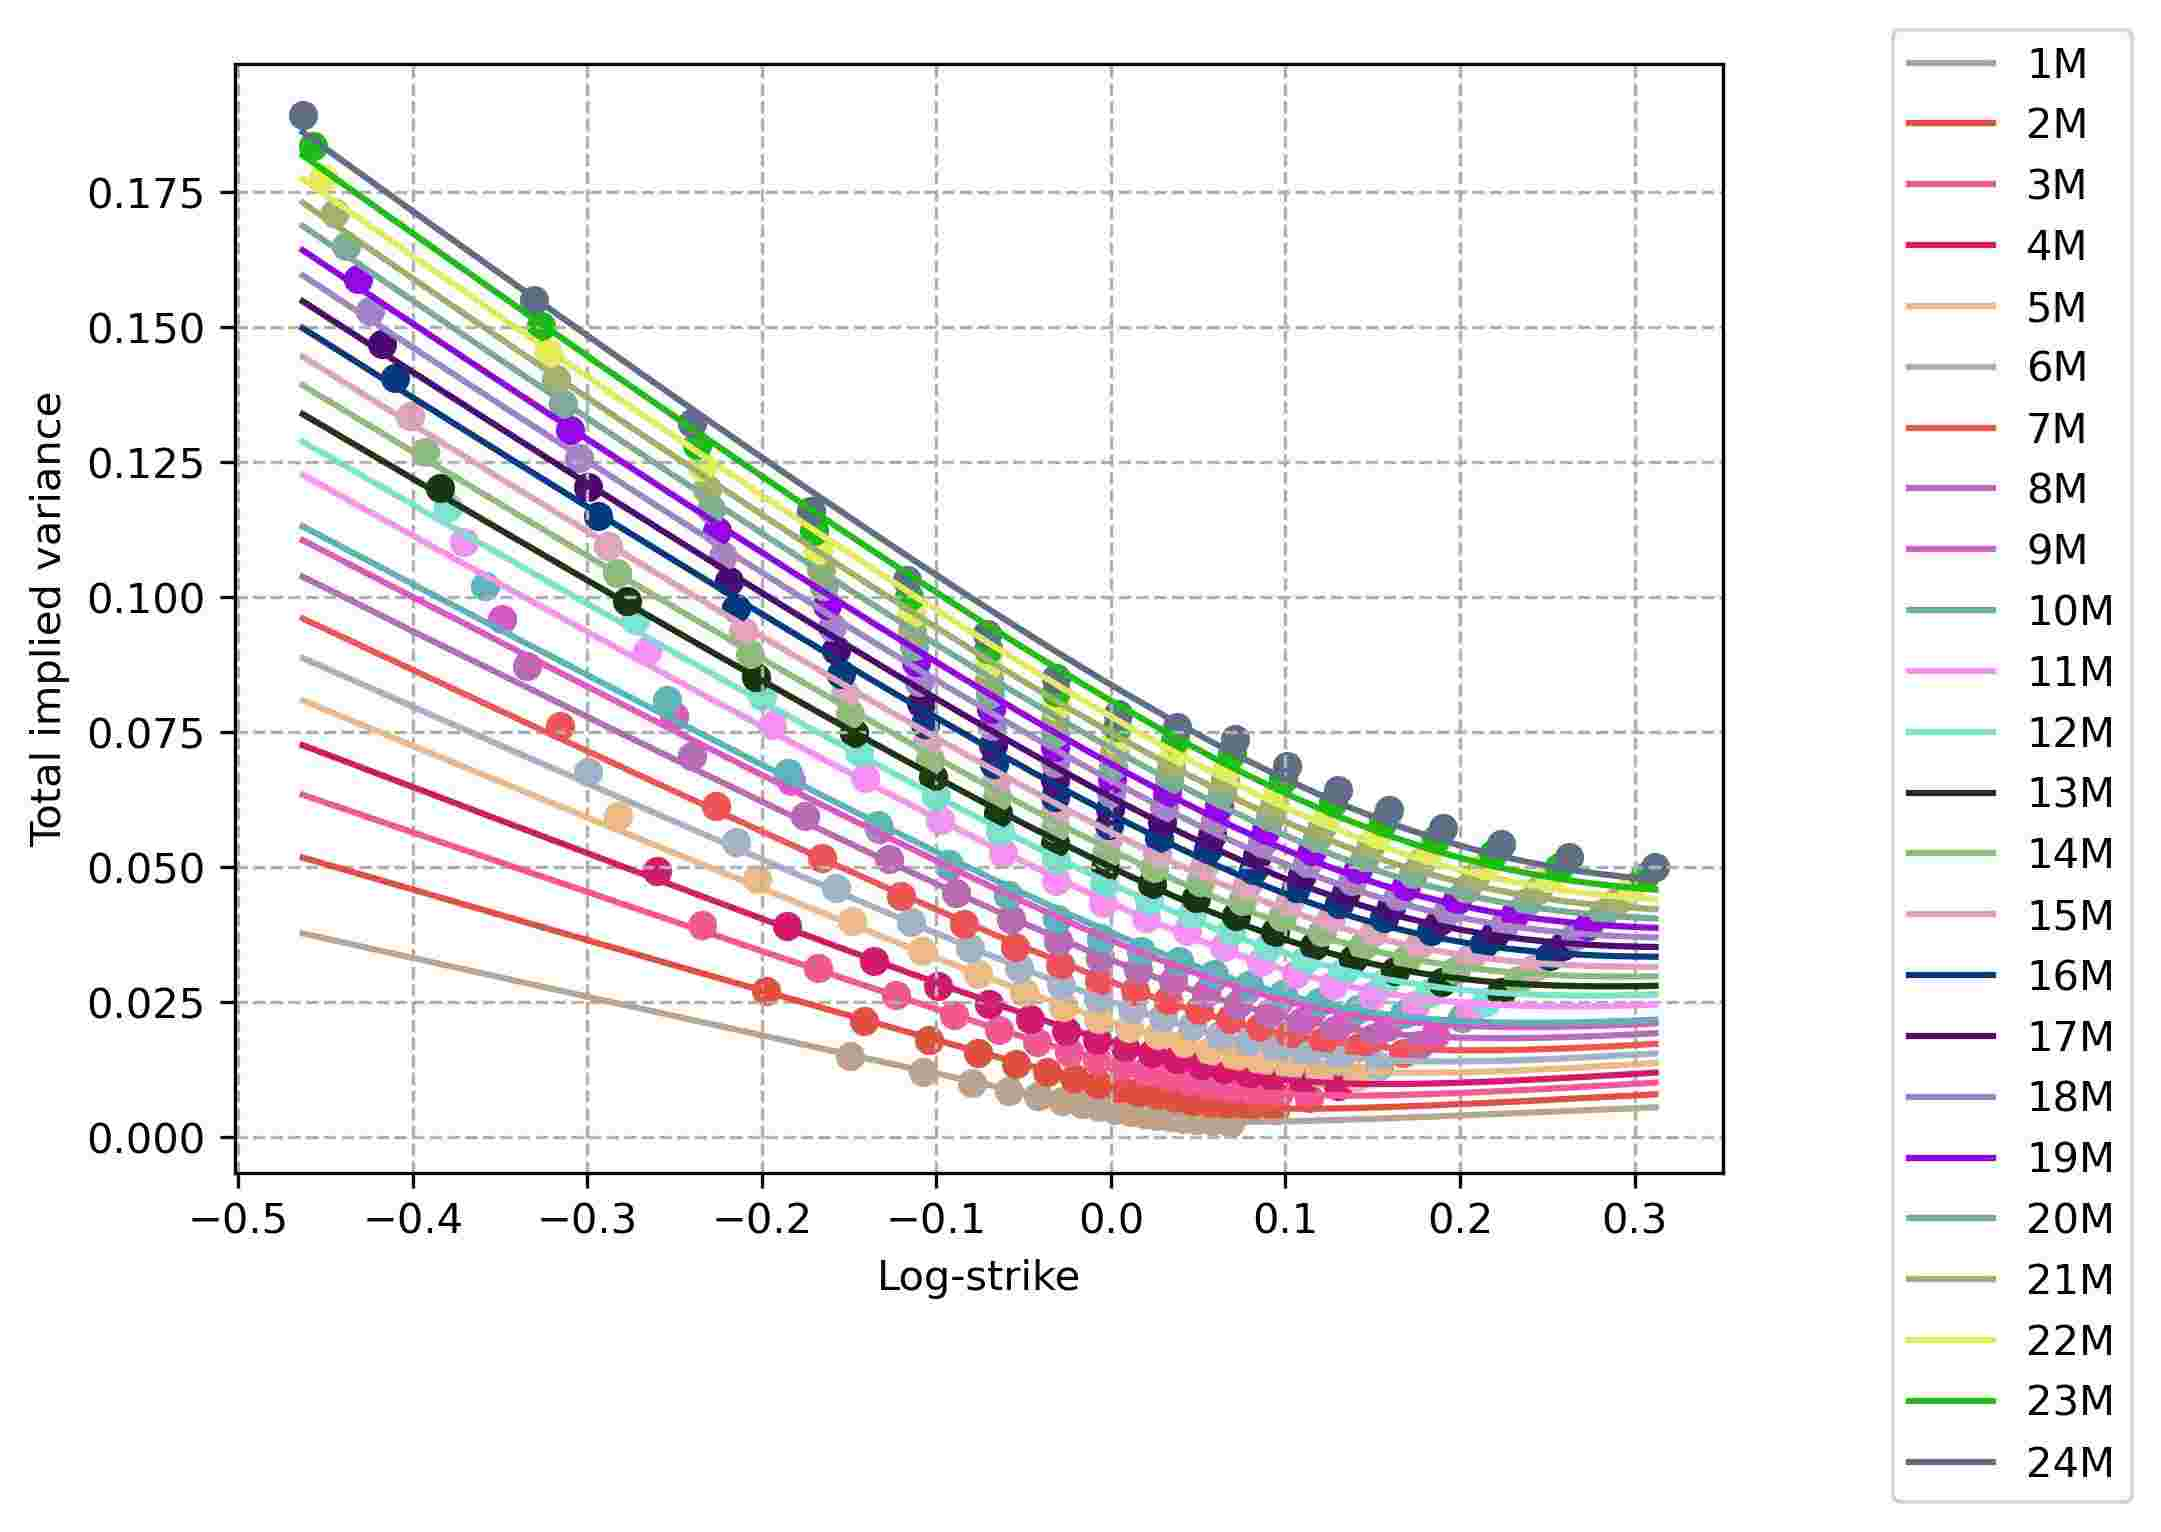
\includegraphics[width=0.45\linewidth]{SX5E_fit_18022022.jpg}}
%     \caption{Illustrations of the fit of the SSVI with the modified power-law parameterization on market total variances for all time-to-maturities. The dots (resp. the lines) correspond to the market (resp. the SSVI) total implied variances.}
% \label{fig:ssvi_replication}
% \end{figure}

At this stage, let us recall that our final objective is to design a model to jointly simulate arbitrage-free IVSs and the price of the underlying asset by simulating the evolution of the SSVI parameters as a function of the path of the underlying asset price. However, the number of parameters involved is so large (there are $n+2$ parameters for the SSVI-HL and $n+3$ for the SSVI-PL and the SSVI-MPL to fit an IVS with $n$ maturities) that a model for their joint evolution would be too complicated. Therefore, we need to make the SSVI model more parsimonious. We propose the two following simplifications:
\begin{enumerate}
    \item We consider only the modified power-law parameterization with $\gamma$ fixed to 1/2 because we observe that $\gamma$ is close to this value over the two data sets (more than 84\% of the calibrated $\gamma$'s lie within the $[0.4,0.6]$ interval). Moreover, this choice has the advantage of guaranteeing that the full surface (without any restriction on the ATM total implied variance) is free of static arbitrage on the sole condition that $\eta^2(1+|\rho|) < 4$ (see case (\ref{prop:pssvi_no_arbitrage}) of Proposition \ref{prop:modified_power_law}). Finally, according to Remark \ref{rk:atm_skew}, setting $\gamma=1/2$ implies a power-law decay of the ATM volatility skew which is a relevant property to capture.
    \item We assume that $\theta_T = aT^p$ where $a,p\ge 0$ reducing considerably the number of parameters while ensuring that the no-arbitrage constraint on the ATM total variance is always satisfied ($\partial_T\theta_T \ge 0$). This parametric form is inspired by the calibrated vectors $(\theta_{T_i})_{i=1,\dots,M}$ that exhibit almost a linear behavior with the maturity $T$. 
    In Figure \ref{fig:theta_t}, we show how this parametric form fits the ATM total variances for several dates. Note that the parameters $a$ and $p$ that have been used in this figure are those calibrated on the whole IVS so the quality of the fit is reduced in comparison to a calibration on the ATM volatilities only. Despite this, the fit is overall satisfying. 
\end{enumerate}
\begin{figure}[h]
    \centering
    \subfigure[S\&P 500 ]{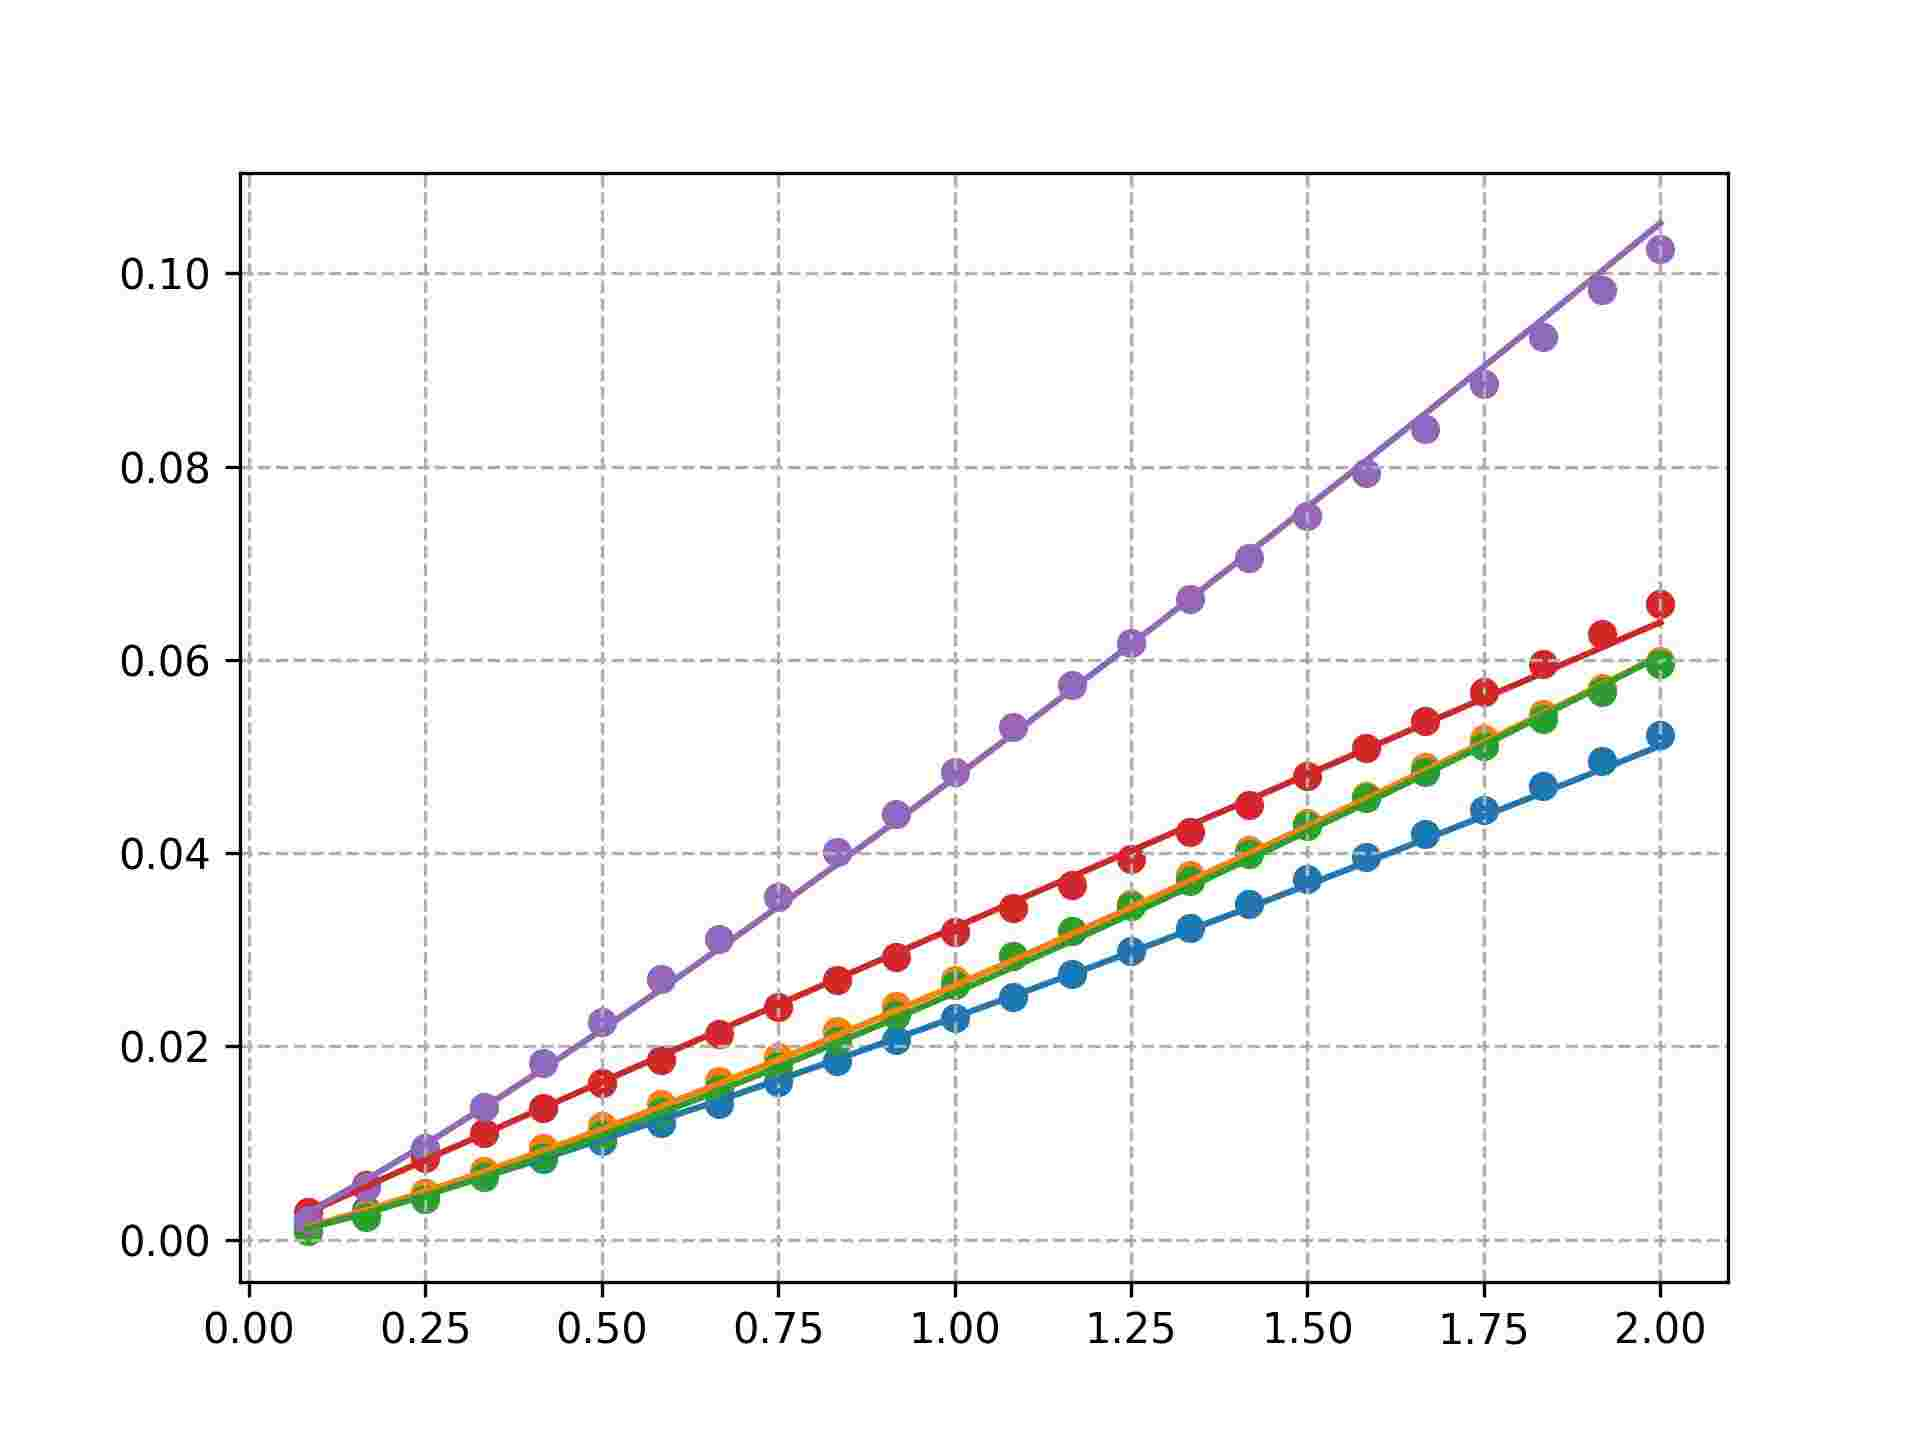
\includegraphics[width=0.45\linewidth]{SPX_theta_T_close_to_mean.jpg}}
    \subfigure[Euro Stoxx 50]{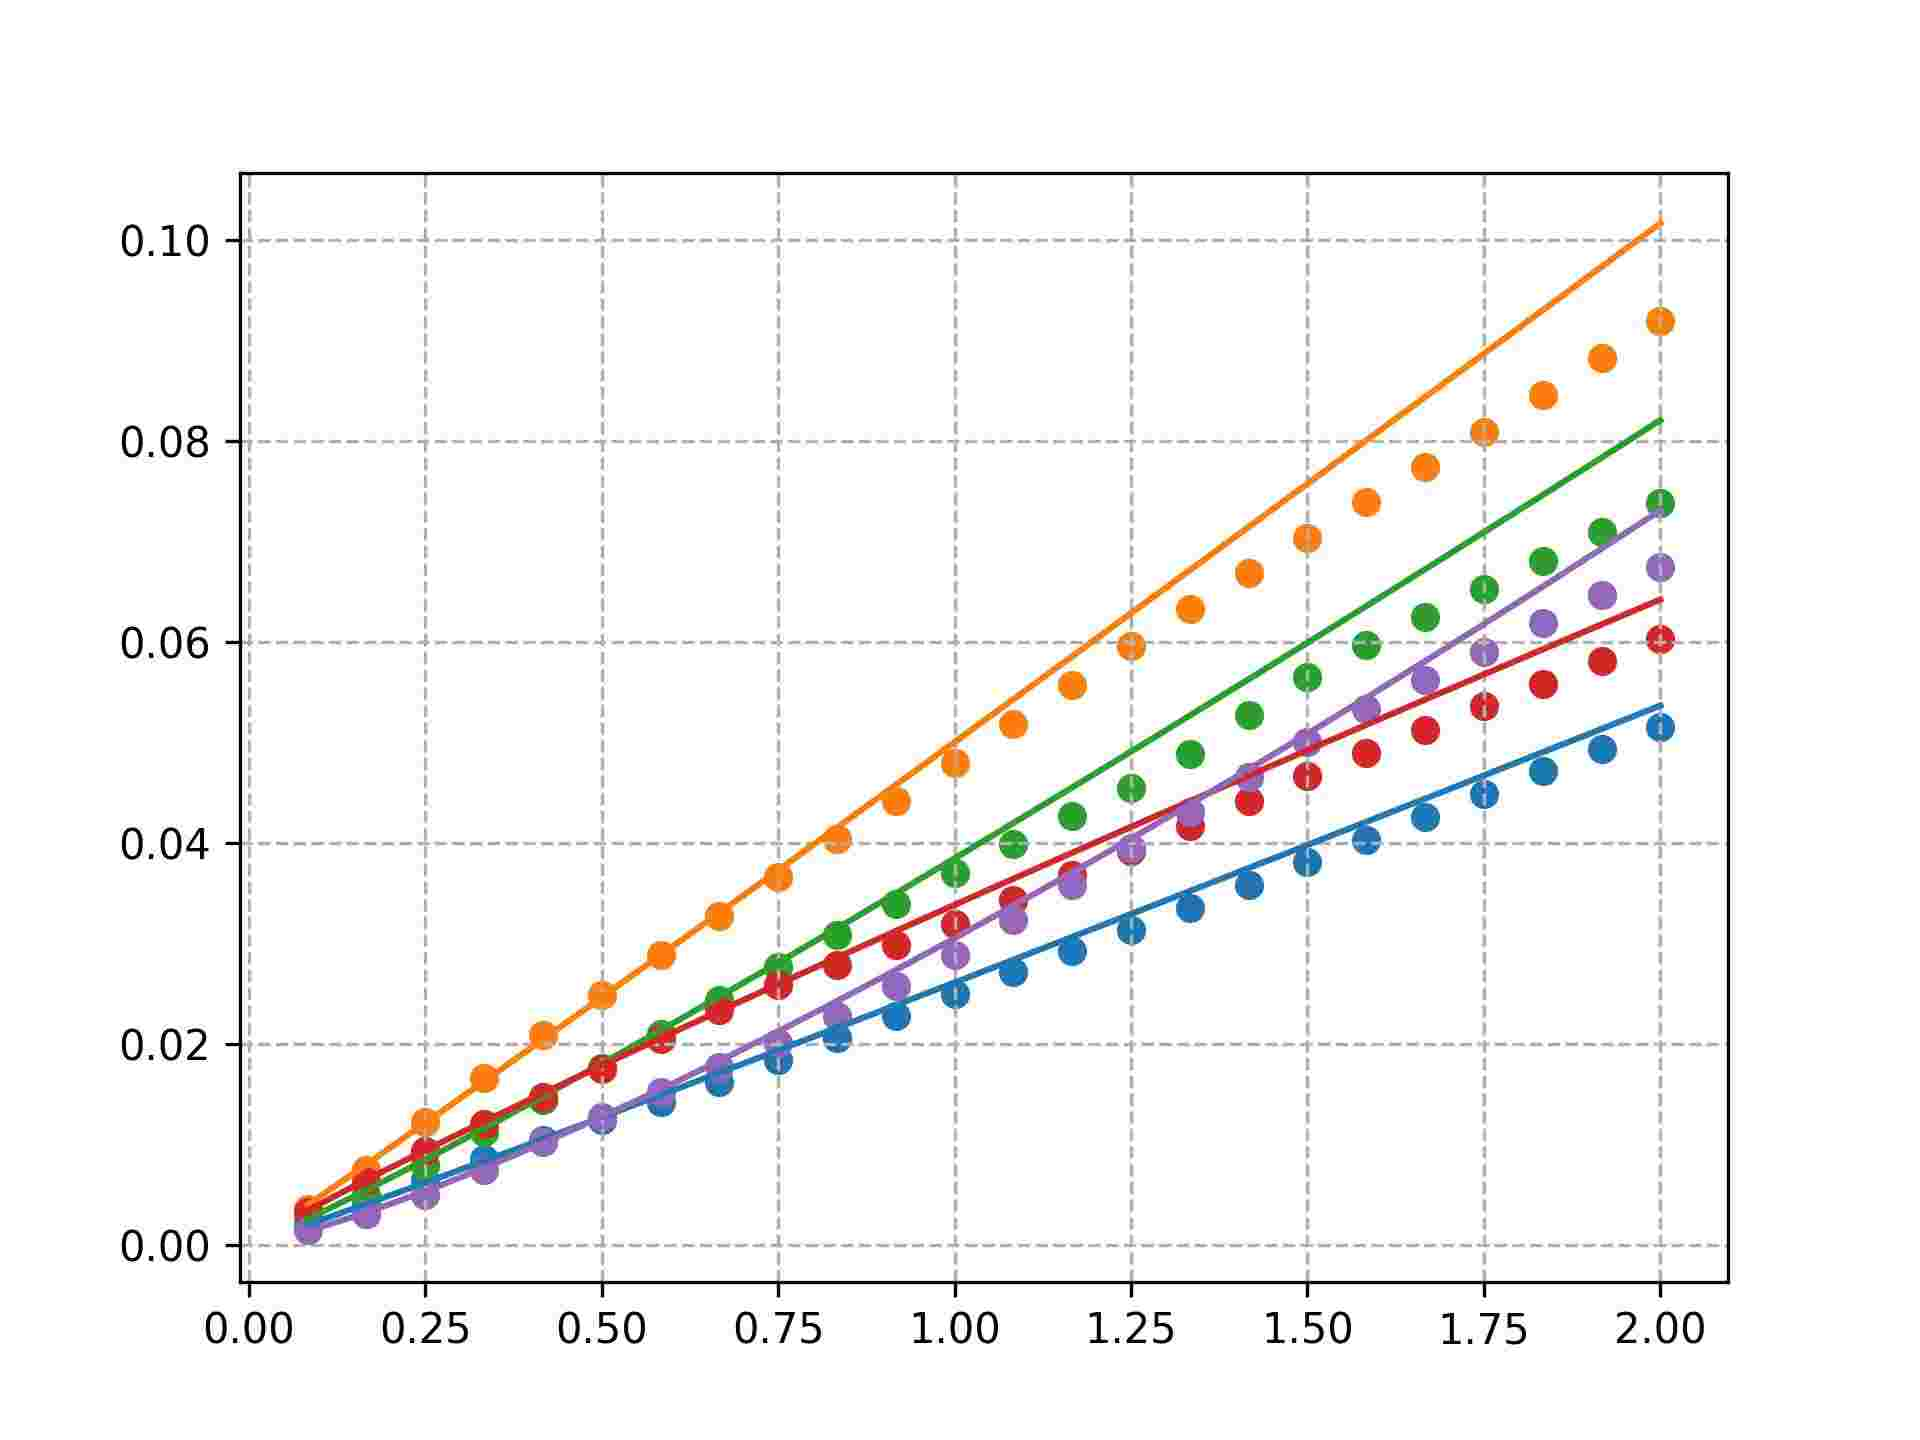
\includegraphics[width=0.45\linewidth]{SX5E_theta_T_close_to_mean.jpg}\label{fig:theta_t_worst_case}}
    \caption{Comparison of the S\&P 500 ATM total variances (dots) with the fitted parametric form $T\mapsto aT^p$ (lines) for five dates (each color corresponds to one date). The five dates are those where the average relative error is the closest to the mean over all average relative errors.}
\label{fig:theta_t}
\end{figure}

The new model obtained after these simplifications is called thereafter the parsimonious SSVI model.
\begin{definition}[Parsimonious SSVI]\label{def:parsimonious_ssvi}
    The parsimonious SSVI is the parameterization of the total implied volatility surface defined by:
\begin{equation}
    w(k,T) = \frac{\theta_T}{2}\left(1+\rho\varphi(\theta_T)k+\sqrt{(\varphi(\theta_T)k+\rho)^2+(1-\rho^2)} \right).
\end{equation}  
where $\theta_T = aT^p$ and $\varphi(\theta) = \frac{\eta}{\sqrt{\theta(1+\theta)}}$ with $a,p\ge 0$ and $\eta>0$. 
\end{definition}

In Figure \ref{fig:parsimonious_ssvi_relative_error}, the average relative errors between the market implied volatilities and the SSVI implied volatilities for each day of our data sets obtained for the parsimonious SSVI model are compared to those obtained for the SSVI model with the modified power-law parameterization. In Figure \ref{fig:parsimonious_ssvi_price_error}, we also show the average errors between the market call prices and the SSVI call prices\footnote{The call prices are computed assuming zero interest rate and no dividend.} in basis points (bps) of the spot price. 
\begin{figure}[h]
    \centering
    \subfigure[S\&P 500]{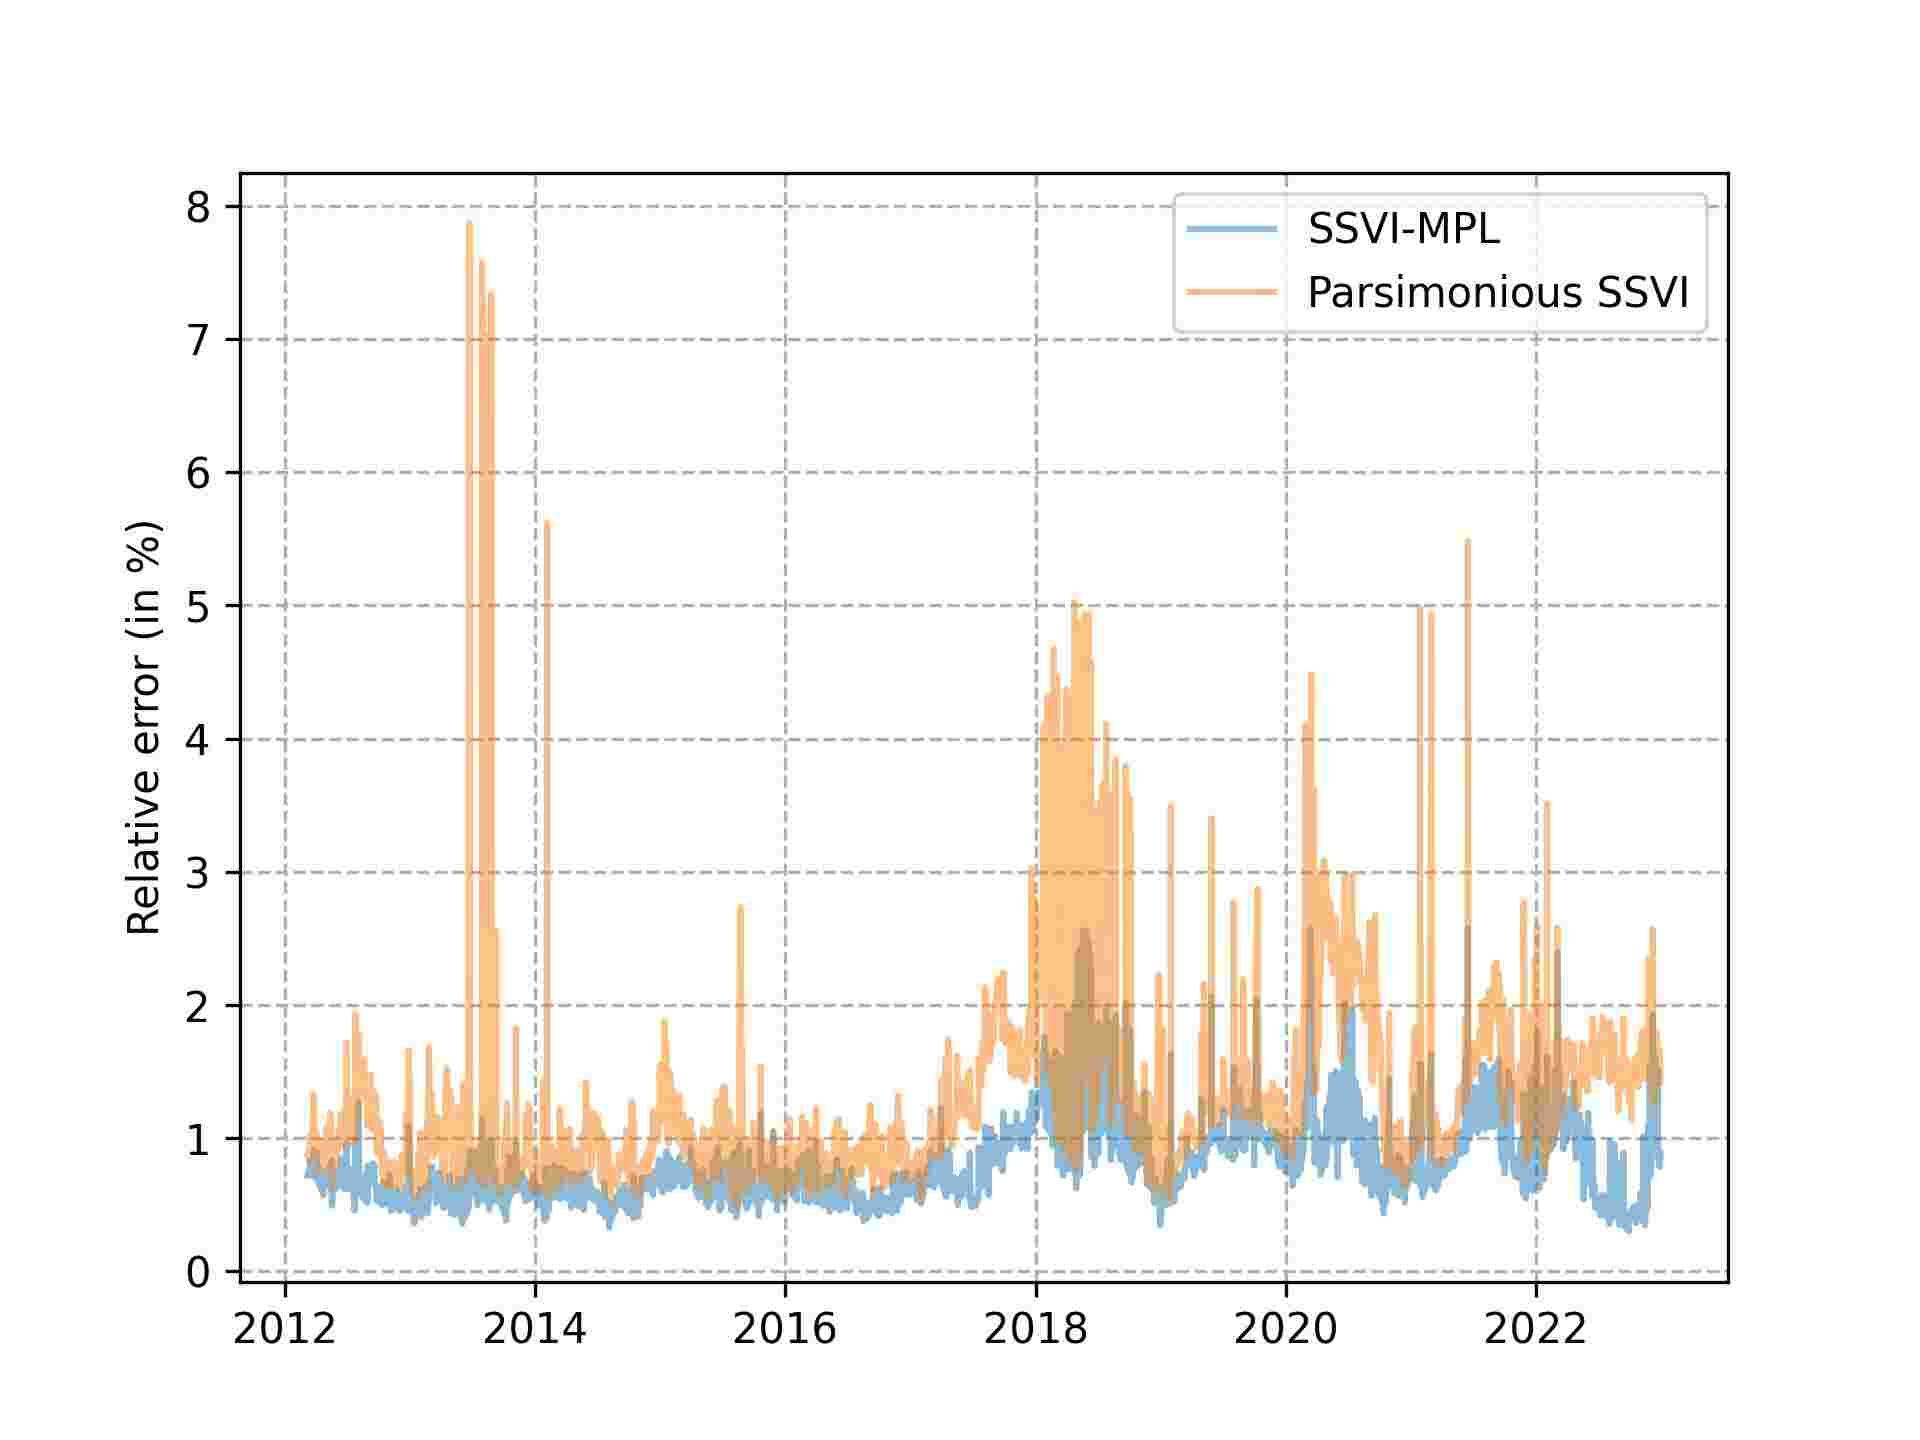
\includegraphics[width=0.45\linewidth]{SPX_parsimonious_SSVI_calibration.jpg}\label{fig:parsimonious_ssvi_relative_error_spx}}
    \subfigure[Euro Stoxx 50]{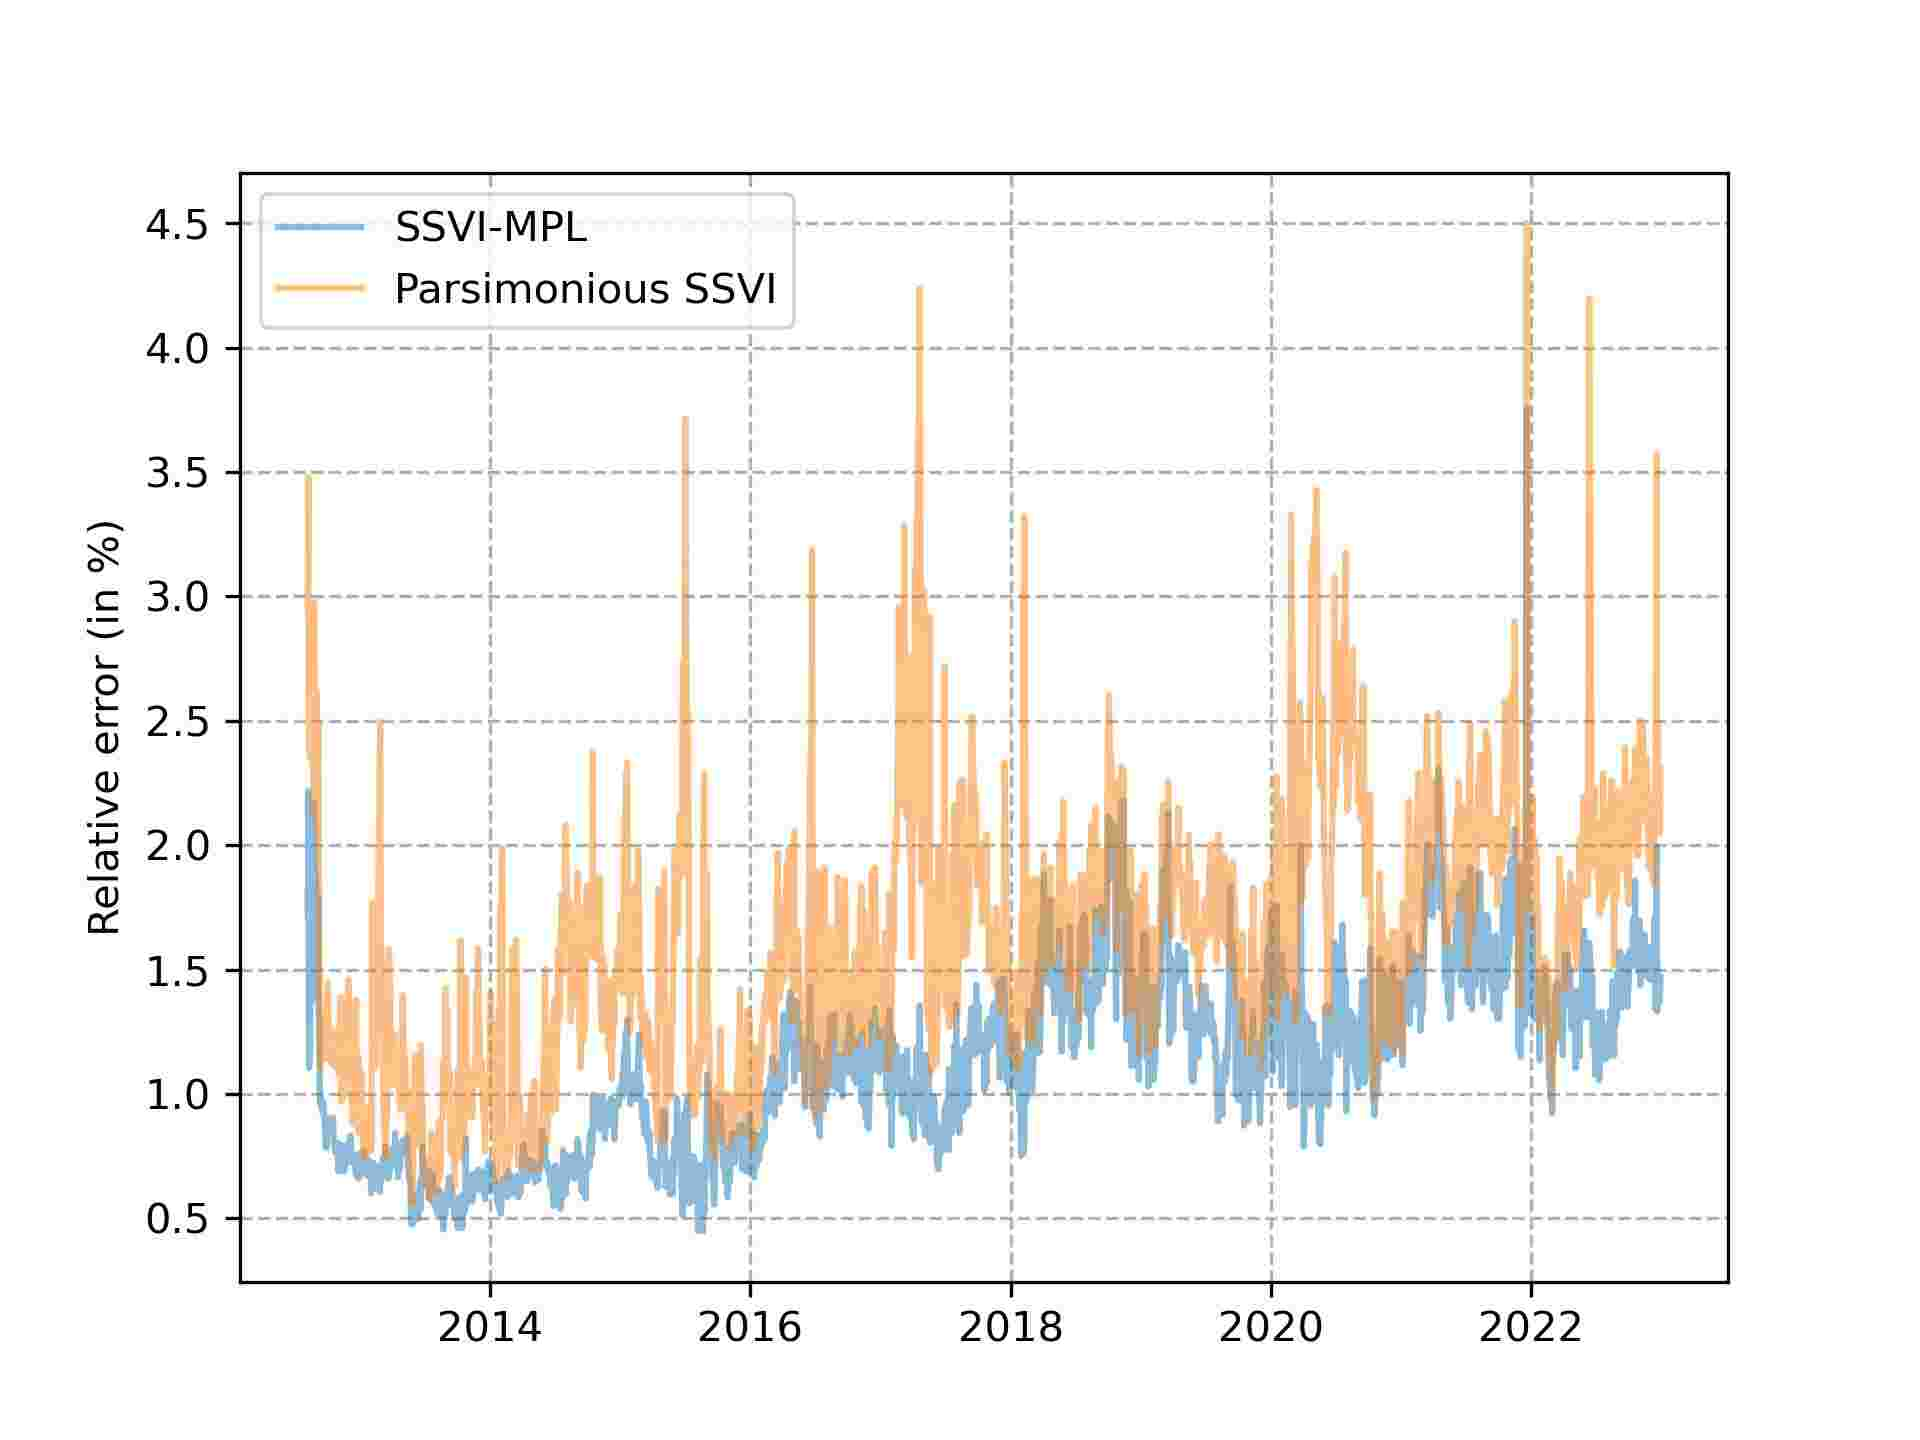
\includegraphics[width=0.45\linewidth]{SX5E_parsimonious_SSVI_calibration.jpg}}
    \caption{Average relative errors between the market implied volatilities and the SSVI implied volatilities for the parsimonious SSVI model and the SSVI-MPL model.}
\label{fig:parsimonious_ssvi_relative_error}
\end{figure}
\begin{figure}[h]
    \centering
    \subfigure[S\&P 500]{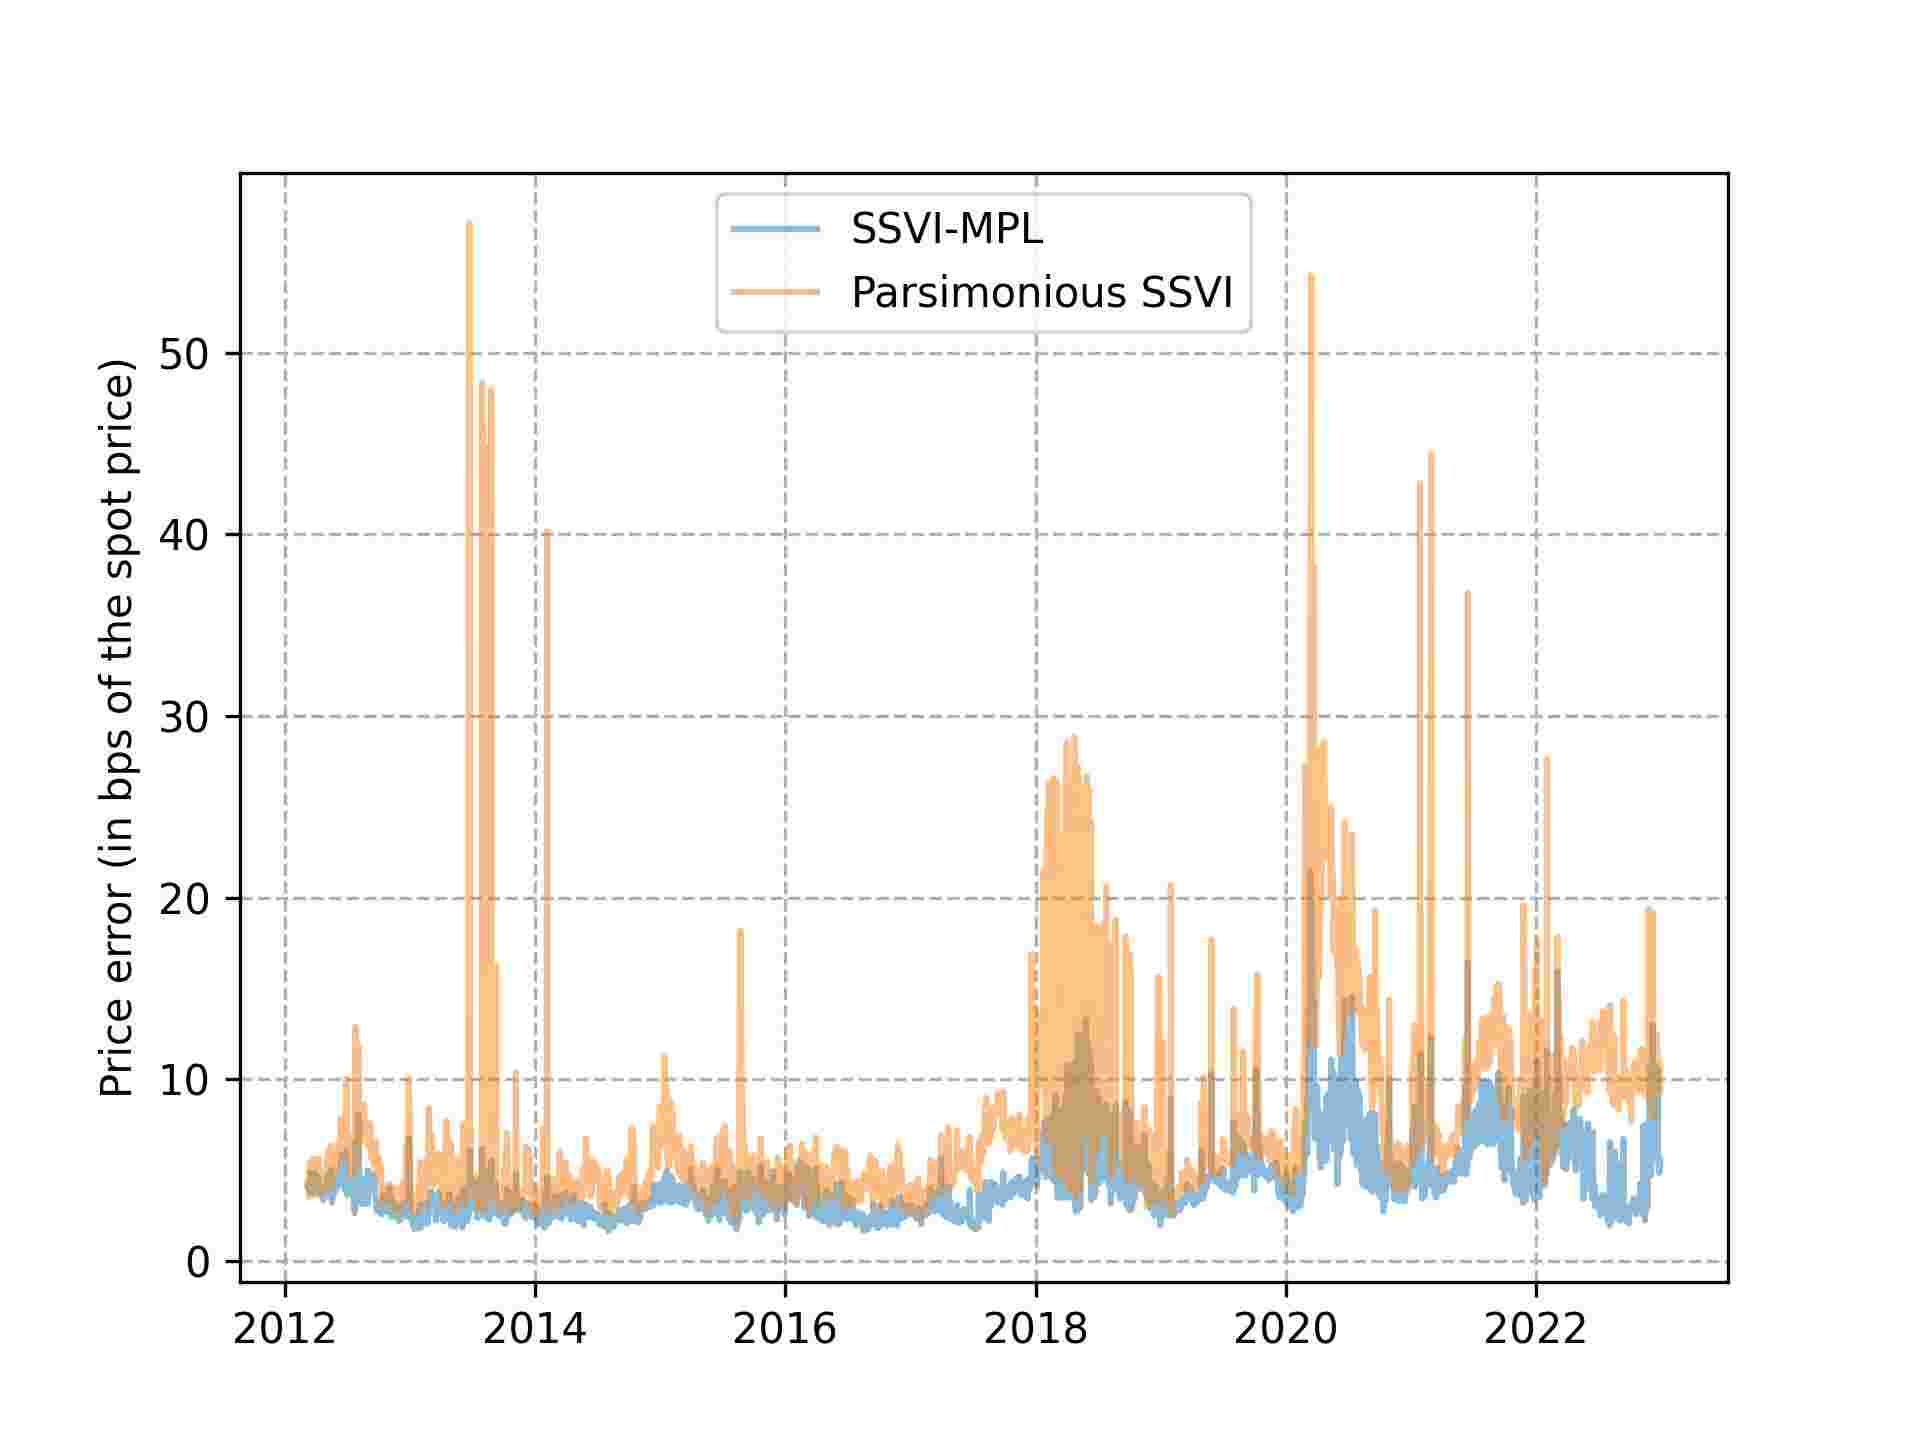
\includegraphics[width=0.45\linewidth]{SPX_parsimonious_SSVI_calibration_Price.jpg}}
    \subfigure[Euro Stoxx 50]{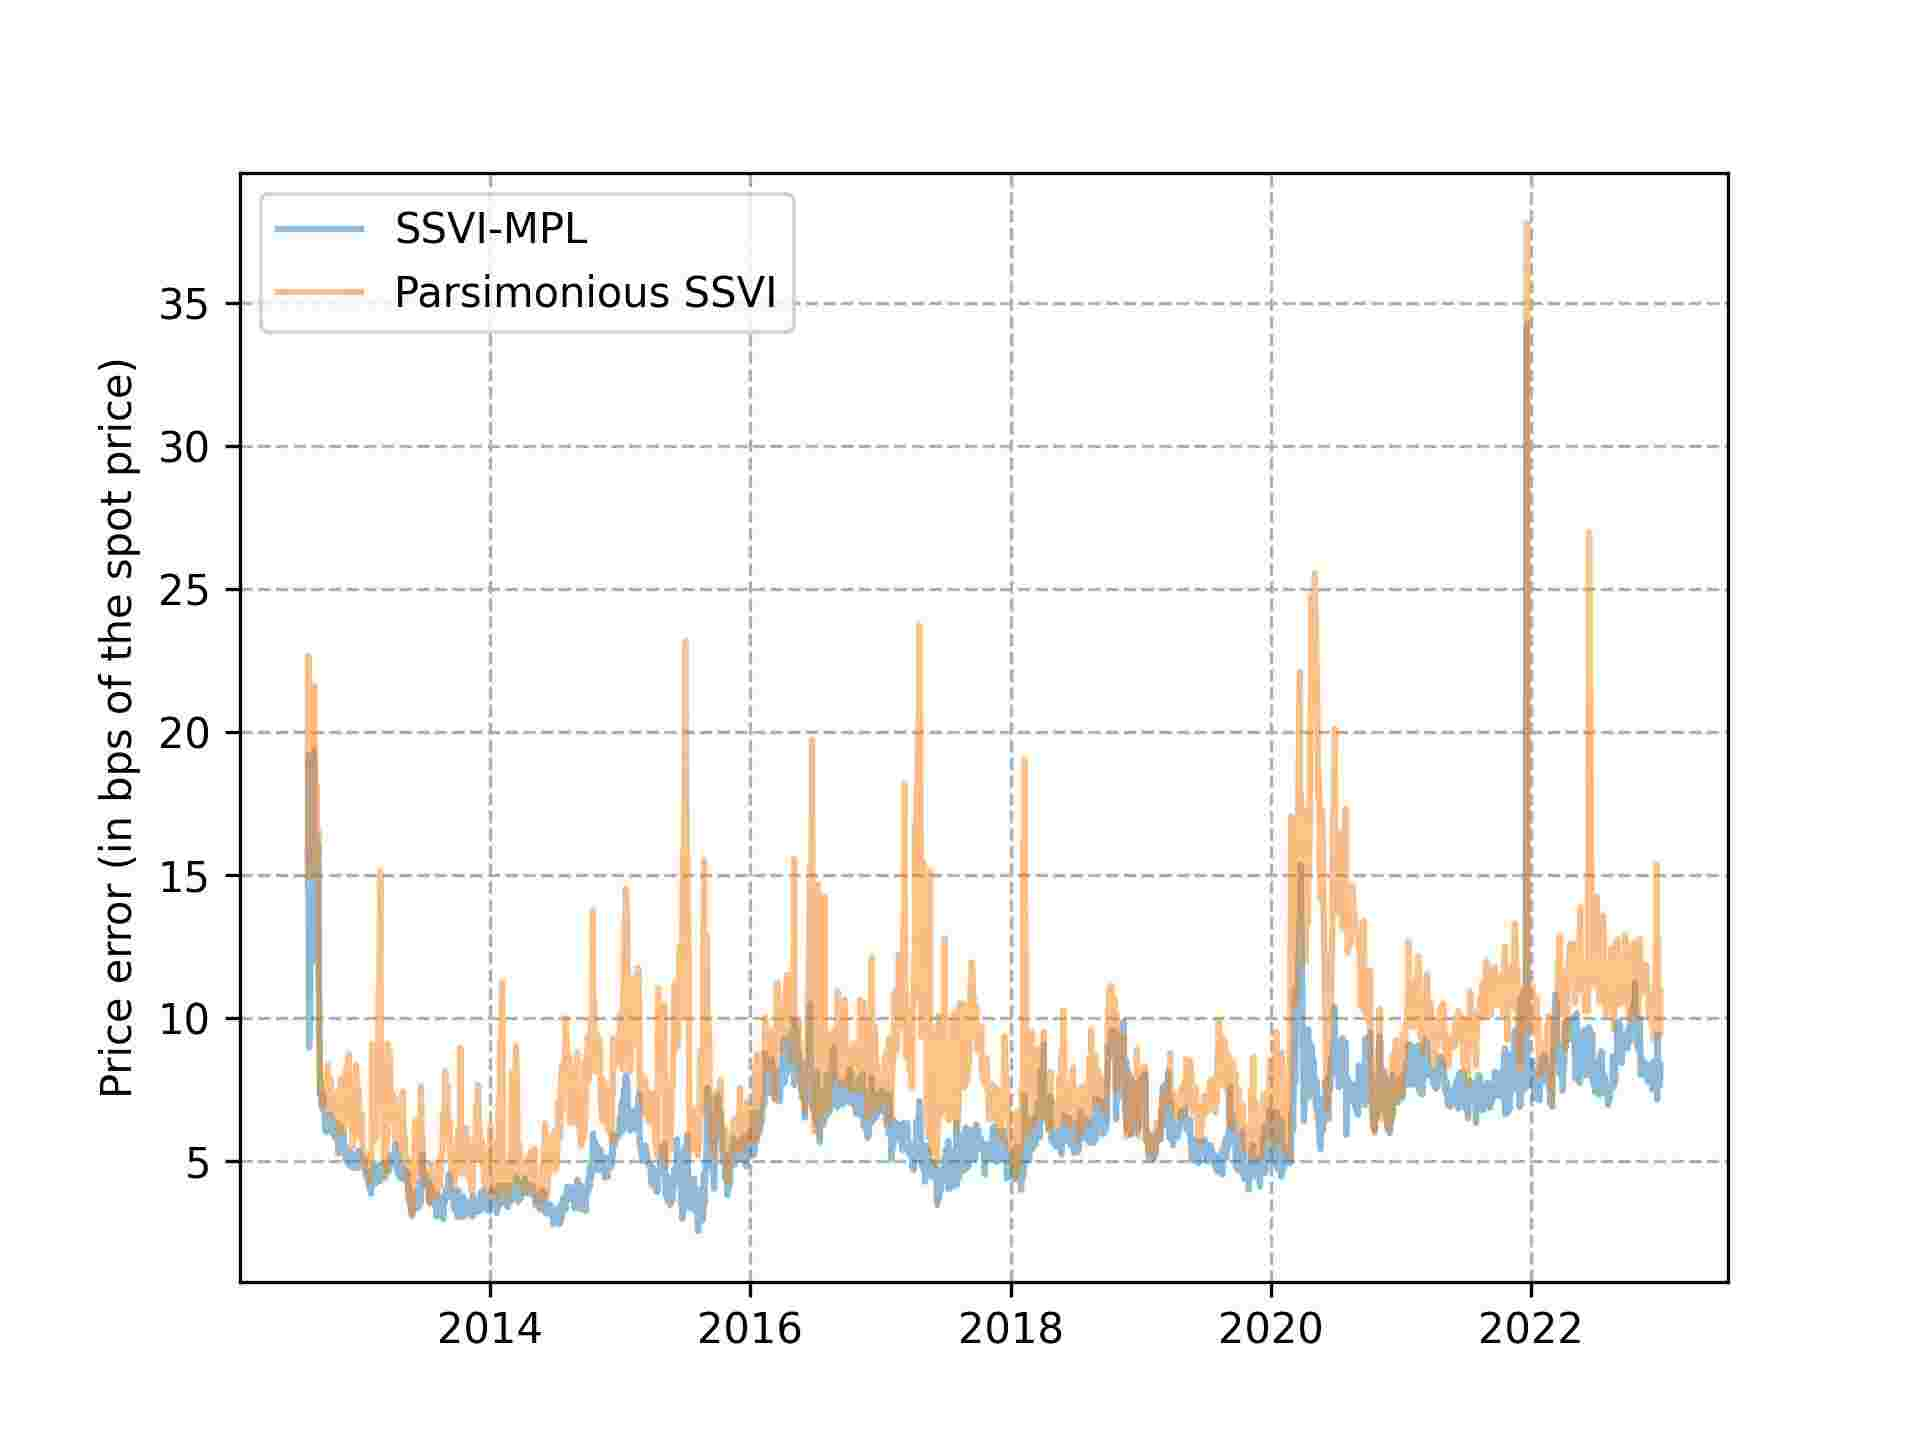
\includegraphics[width=0.45\linewidth]{SX5E_parsimonious_SSVI_calibration_Price.jpg}}
    \caption{Average price errors between the market call prices and the SSVI call prices for the parsimonious SSVI model and the SSVI-MPL model.}
\label{fig:parsimonious_ssvi_price_error}
\end{figure}

As expected, the calibration accuracy is reduced for the parsimonious SSVI. However, it remains overall quite close to the SSVI-MPL calibration in view of the reduction of the number of parameters: 4 parameters for the parsimonious SSVI versus 27 for the SSVI-MPL. The mean of the average relative errors across the whole S\&P 500 (resp. Euro Stoxx 50) data set increases from 0.80\% (resp. 1.18\%) to 1.29\% (resp. 1.60\%). Besides, the mean of the average price errors accross the whole S\&P 500 (resp. Euro Stoxx 50) data set increases from 4 bps (resp. 6 bps) to 7 bps (resp. 8 bps).  In our numerical experiments, we observed that the parametric form for $\theta_T$ is the assumption leading to the largest deterioration of the fit to market implied volatilities, which is consistent with the fact that this assumption is the one limiting the most the number of degrees of freedom of the model. In Figure \ref{fig:pssvi_fit}, we illustrate how the parsimonious SSVI fits the S\&P 500 (resp. the Euro Stoxx 50) total implied variances for a day where the calibrated average relative error is equal to 1.29\% (resp. 1.60\%) corresponding to the mean of the average relative errors across the whole S\&P 500 (resp. Euro Stoxx 50) data set. 
\begin{figure}[h]
    \centering
    \subfigure[S\&P 500 (February 12, 2021)]{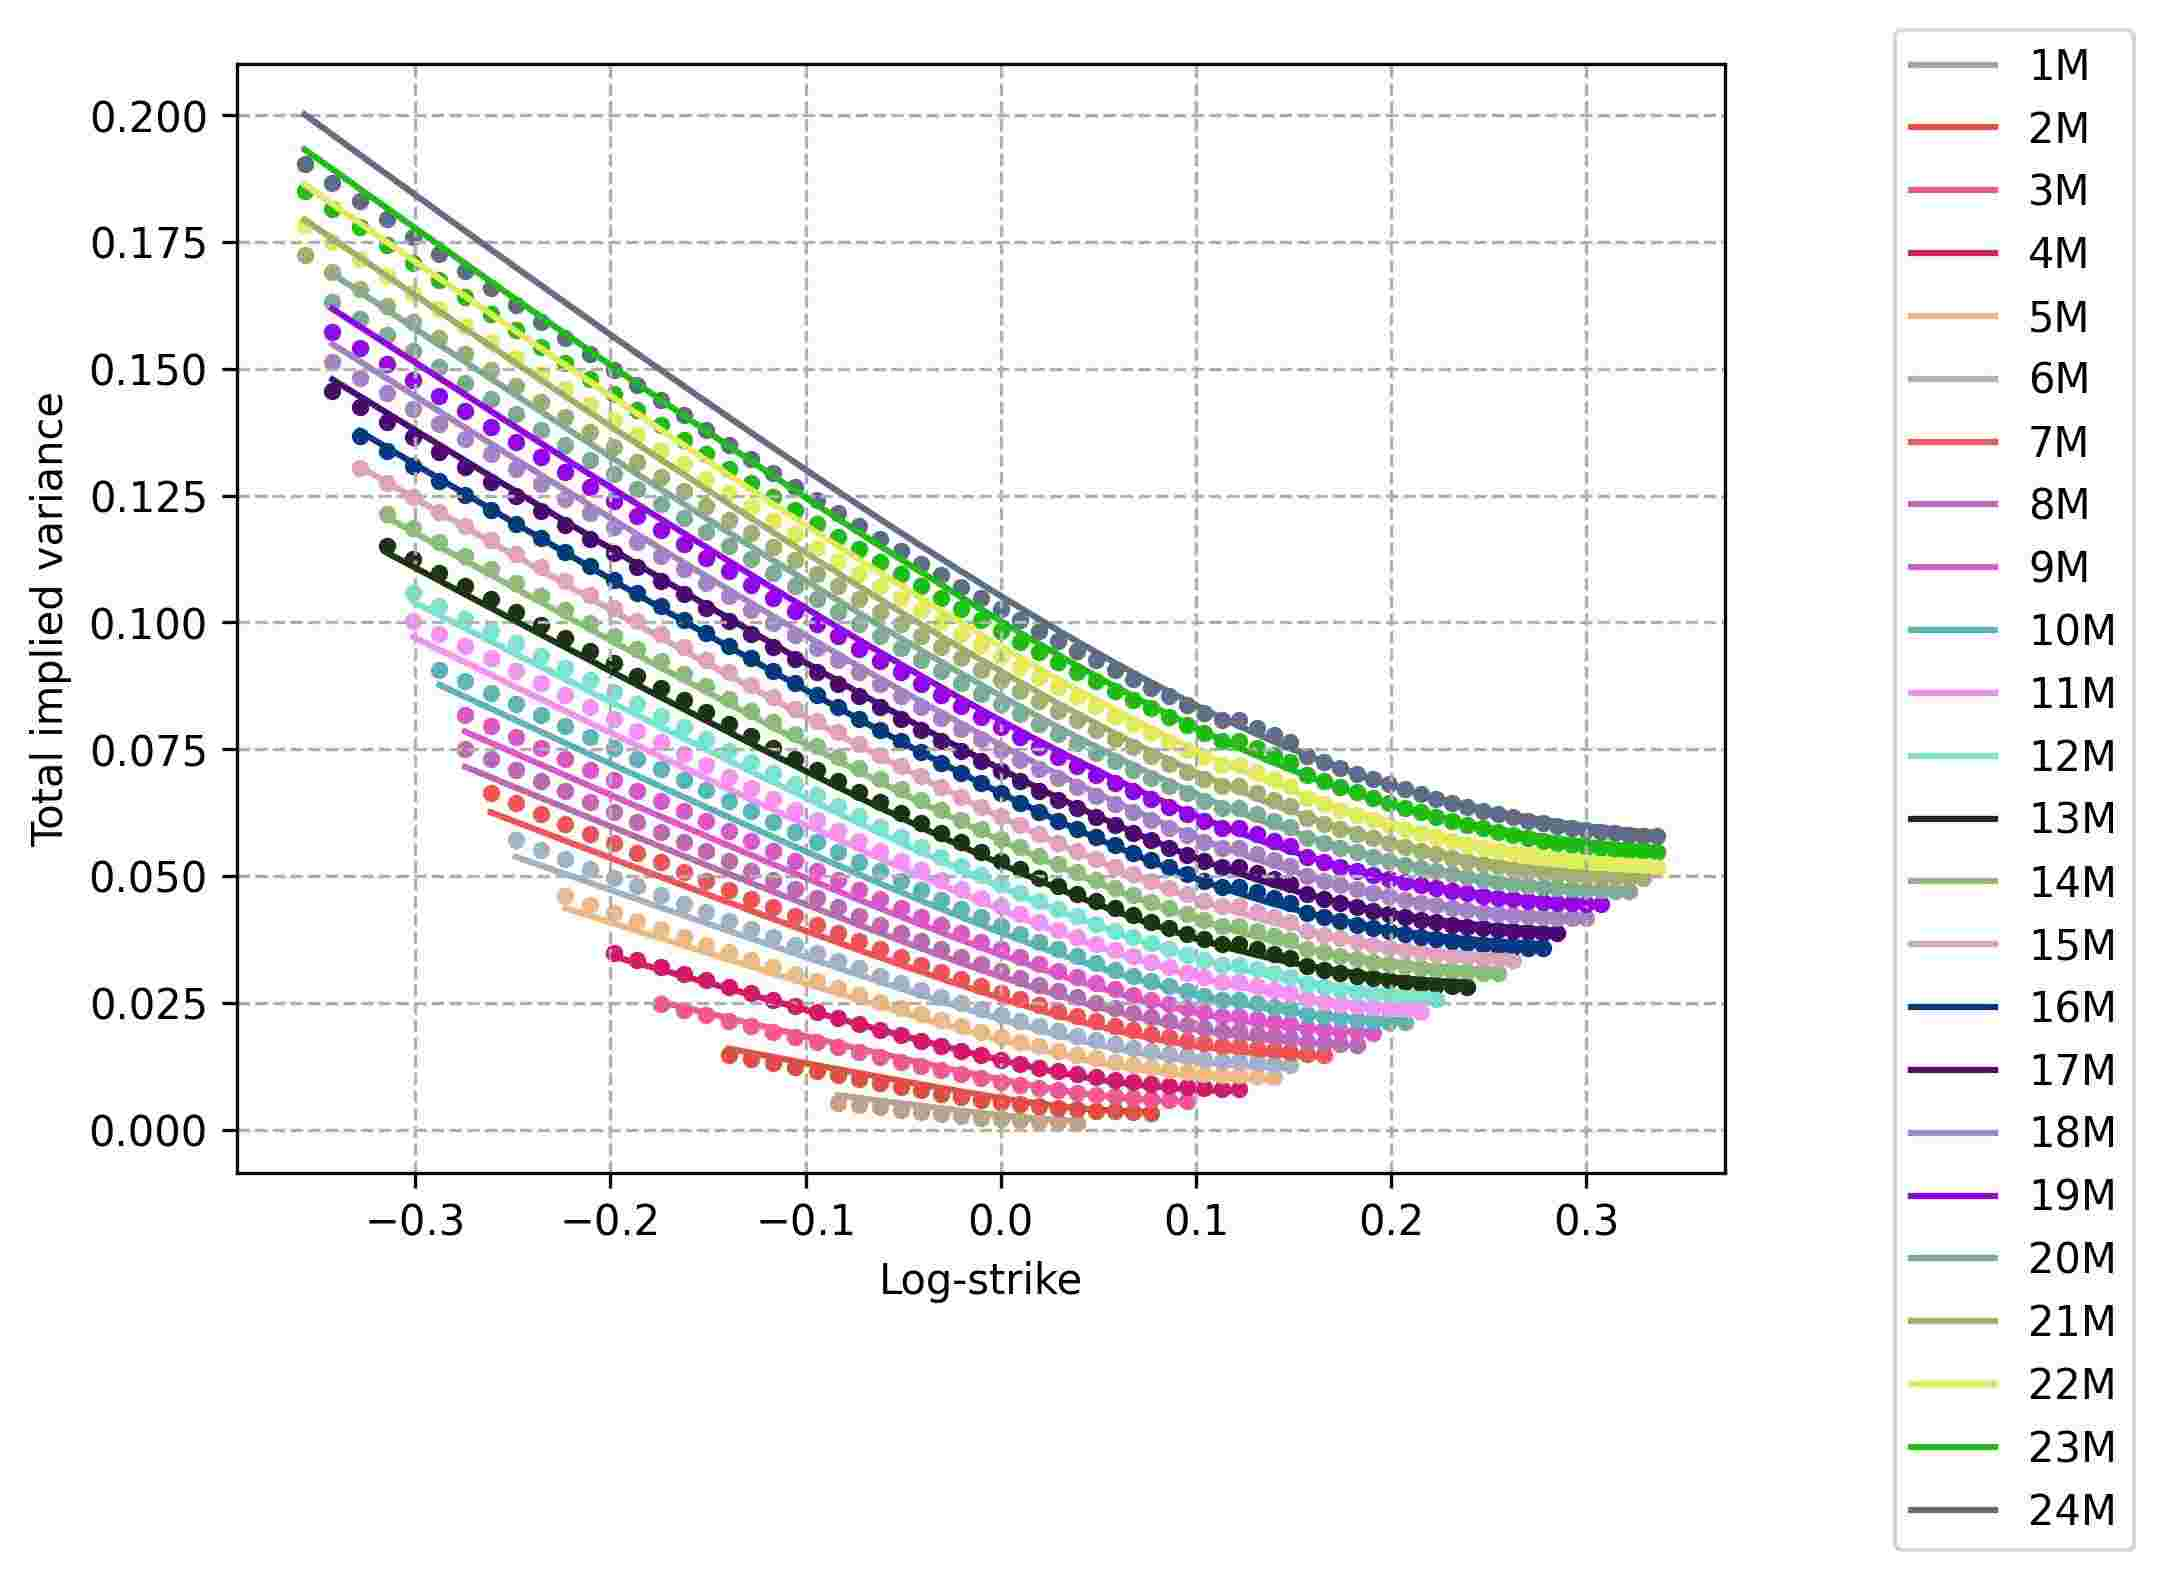
\includegraphics[width=0.45\linewidth]{SPX_pSSVI_Fit_12022021.jpg}}
    \subfigure[Euro Stoxx 50 (August 30, 2019)]{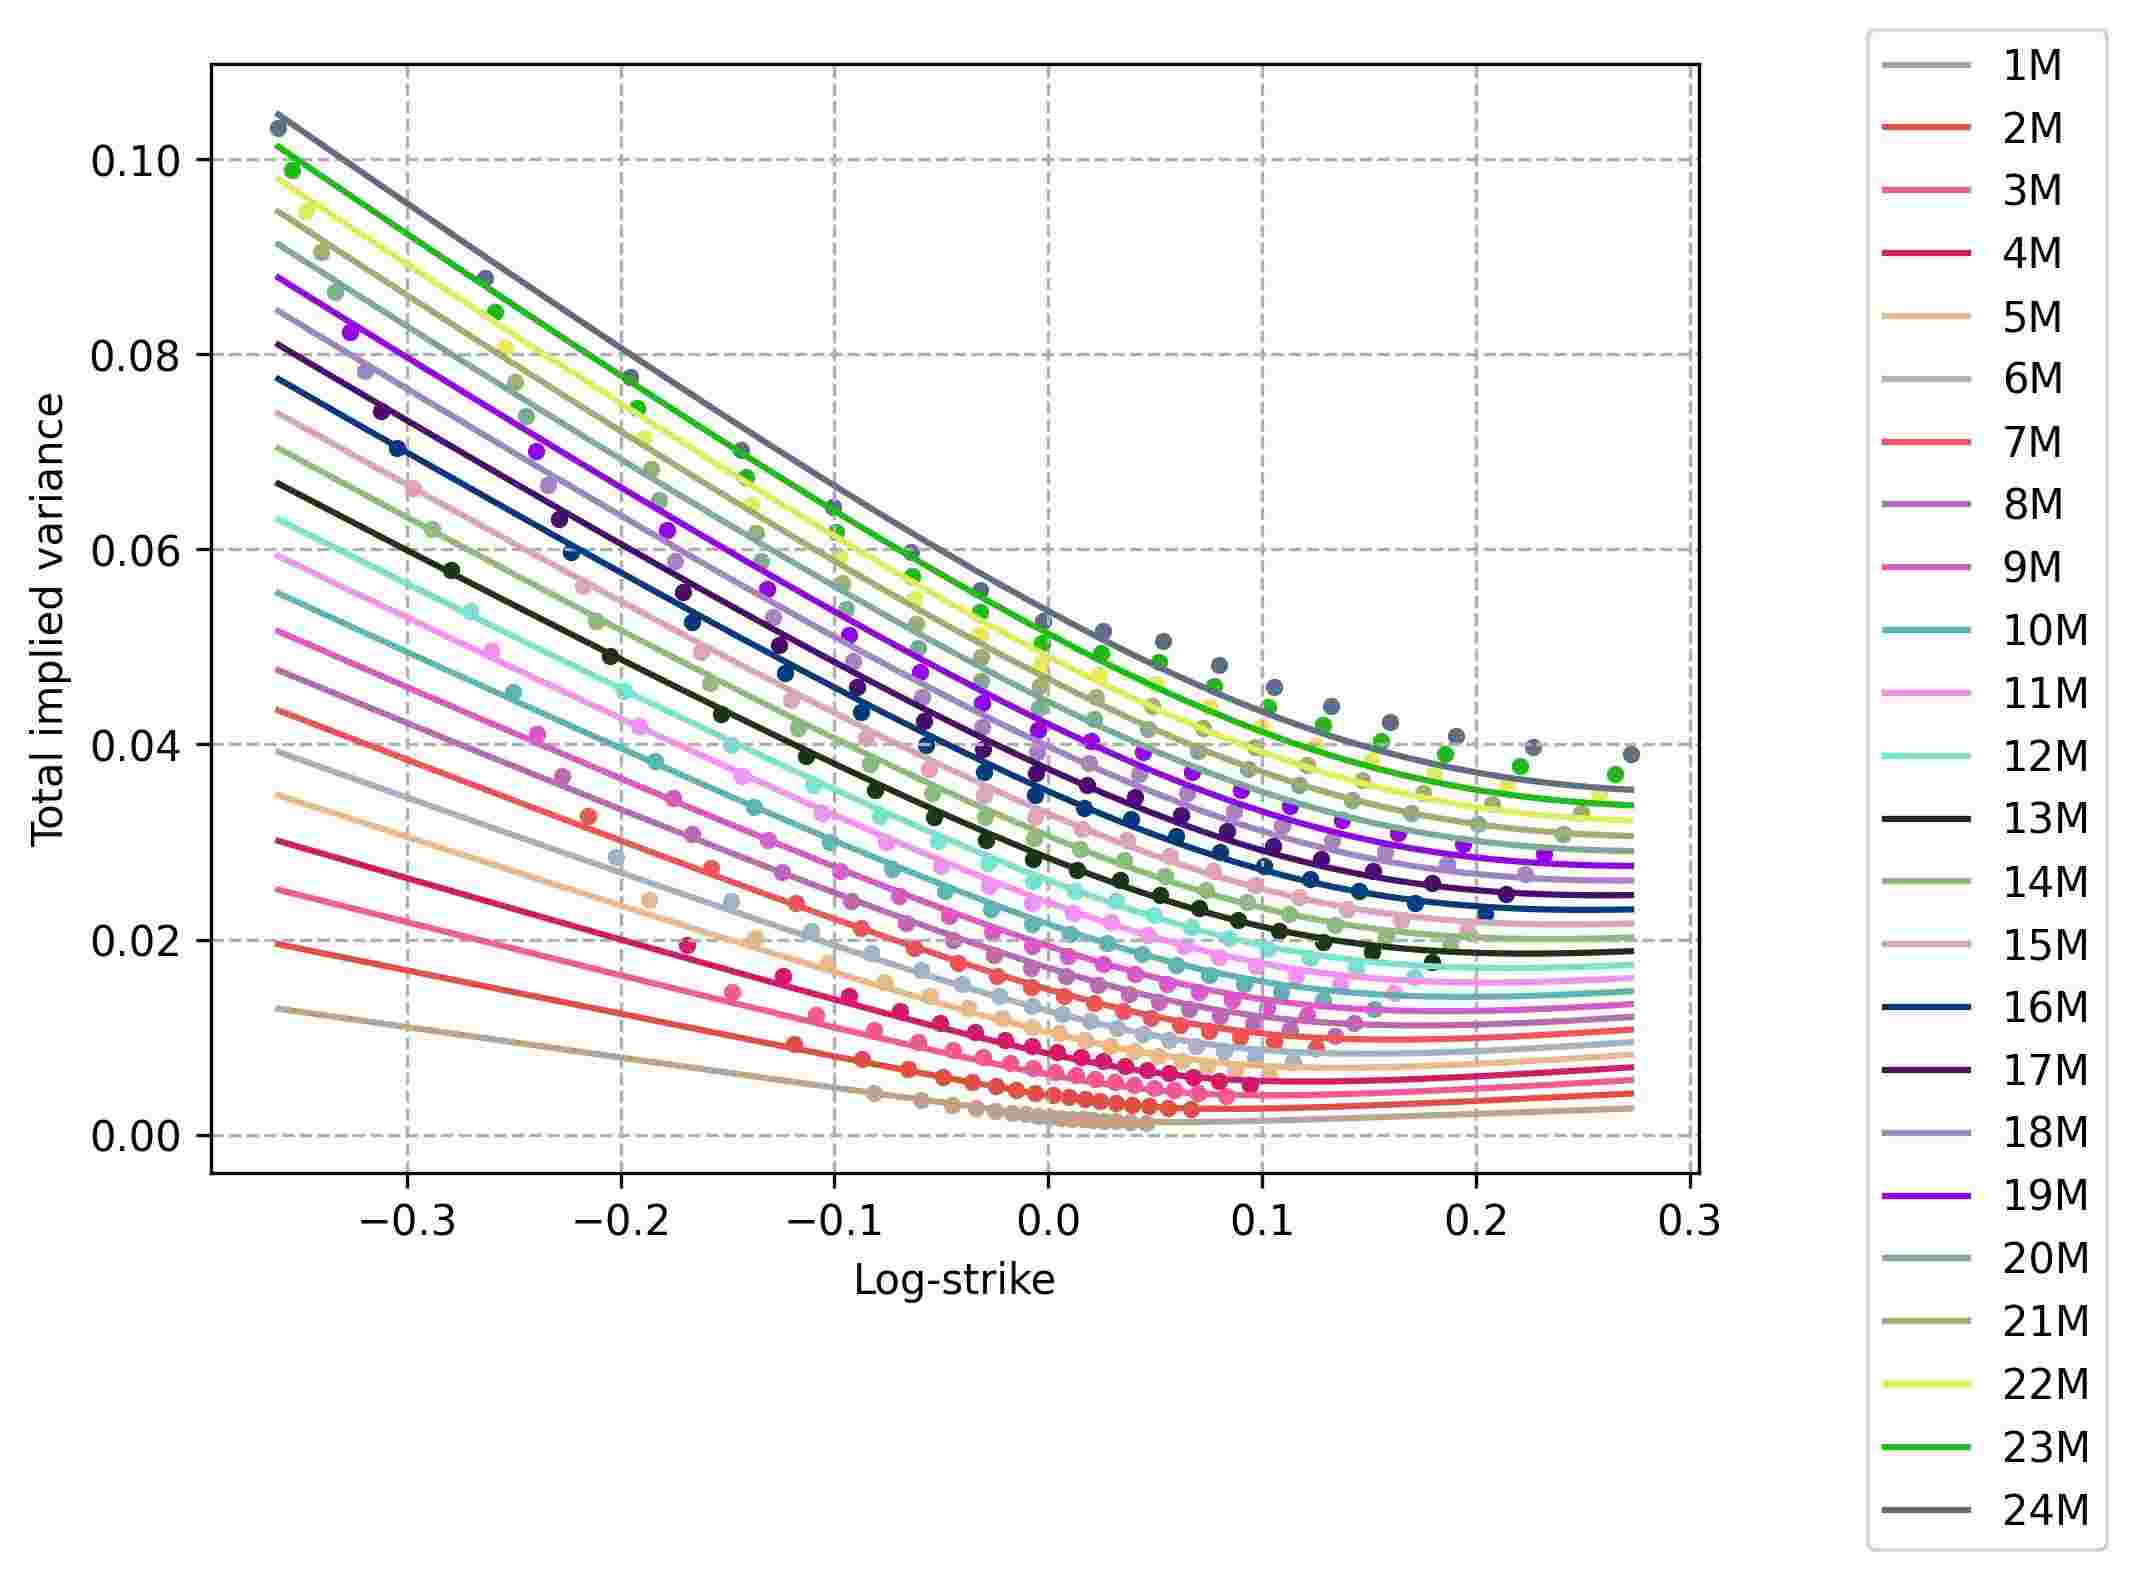
\includegraphics[width=0.45\linewidth]{STXE_pSSVI_Fit_30082019.jpg}}
    \caption{Illustrations of the fit of the parsimonious SSVI on market total variances for all maturities. The dots (resp. the lines) correspond to the market (resp. the SSVI) total implied variances.}
\label{fig:pssvi_fit}
\end{figure}
